\chapter{Concept}

\label{Concept}

The concept chapter of this work gives a brief overview of what components are doing and how they are related. 
A detailed look at each component and its inner workings comes in the following chapters of this work.

%----------------------------------------------------------------------------------------

\section{Workflow Diagram}

\begin{figure}[ht]
	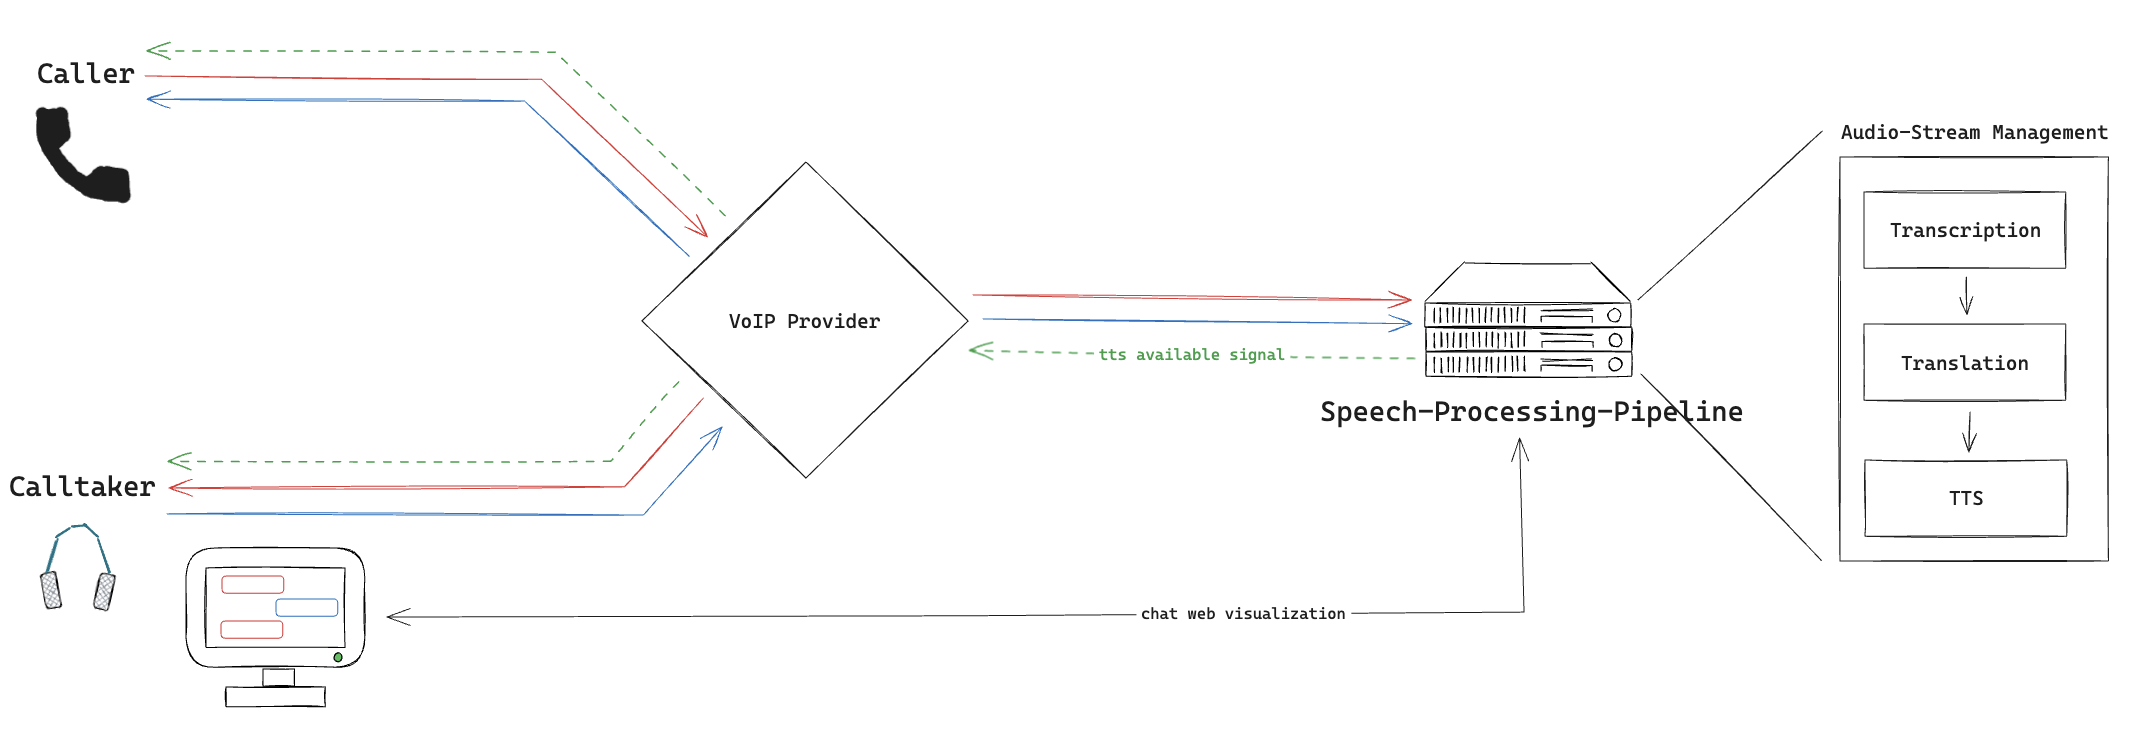
\includegraphics[width=\textwidth]{Figures/data-flow-chart.png}
	\caption{Workflow Diagram}
	\label{fig:workflowDiagram}
\end{figure}

Figure \ref{fig:workflowDiagram} shows a high-level overview of the System's workflow. It shows the phone call between 
the emergency caller and the call-taker. It is routed through the \ac{voip} provider, which forwards the audio stream to 
the speech-processing pipeline server. The server then processes the audio stream by transcribing, translating, and 
synthesizing it. The resulting tts signal gets sent back to the \ac{voip} provider, who plays it back to the caller and 
call-taker, respectively.

The graphic also shows the chat visualization in the web browser. This visualization is optional and can only be used 
by the call-taker in the displayed scenario.

%----------------------------------------------------------------------------------------

\section{Audio Input}

The flexibility of the System allows for various audio input options. This work will cover two of the most important 
ones. The two most critical audio sources are recordings by web browsers and audio input provided by \ac{voip} 
communication systems. This module is described in detail in Chapter \ref{AudioDataReception}.

\subsection{Web Browser Audio}

Within the context of this work, the focus lies on integrating Chromium-based web browsers. The Web MediaRecorder API 
provides the audio input. The API requests access to the microphone and allows for recording audio streams. 
The audio stream gets sent to the server as \ac{webm}-encoded data chunks of about 200ms. The server then concatenates 
the chunks and converts the audio stream to \ac{wav} format. The conversion utilizes FFmpeg, a \ac{cli} tool for 
manipulating audio and video files. The speech-processing pipeline then processes the resulting \ac{wav} file.

\subsection{Voice-over-IP Audio}

To get access to \ac{voip} audio data, a third party gets access to the \ac{api} and forwards the data stream to the 
system. This stream comes via \ac{udp} and contains 20ms of uncompressed \ac{wav} audio data for each chunk.
Each chunk carries an identifiable tag that allows the system to map the audio data against a user.
These chunks get concatenated to be processed by the speech-processing pipeline.

%----------------------------------------------------------------------------------------

\section{Speech Processing}

The speech processing component mainly comprises a microservice wrapping OpenAIs Whisper project. It receives slices of 
the audio stream, various in length, and transcribes them into text. The transcription is then analyzed, and if there 
is no change in content for more than two iterations, it finalizes the pending message. Any new content will cause the 
creation of a new message object, and the process will start over. This module is described in detail in Chapter 
\ref{SpeechProcessing}.

The speech-processing pipeline utilizes Whisper to determine the spoken language as well. It returns the most likely 
language used in the audio file. Alongside the integrated voice-activation feature to filter out sections that do not 
contain spoken content, Whisper is a very versatile tool.

After a message is determined to have ended, the system utilizes DeepL to translate the message into any foreign 
language spoken within the same session, described in detail in Chapter \ref{SessionHandlingAndMessageTranslation}.

%----------------------------------------------------------------------------------------

\section{Session Handling}

After creating a new session with its corresponding ID, users can join it by connecting to it with an audio stream. 
Each audio stream is related to a known Notitia User account or gets a temporary user object. In the latter case, the 
user will not be able to be identified as the same one if the audio connection drops and gets reconnected. 
This module is described in detail in Chapter \ref{SessionHandlingAndMessageTranslation}.

The session object holds various data about the connected audio streams, their users, and the determined spoken 
languages of each one. This data leads to generating the necessary translations of a message. A session is also 
responsible for broadcasting the information about generated audio files to the appropriate receivers.

It is possible to connect any number of users to one singular session. However, within this work, a two-user session is 
most common since it represents the use case of an emergency caller and call-taker.

%----------------------------------------------------------------------------------------

\section{Audio Output}

After the translated text is available, the system can synthesize an audio file. The audio file gets created 
using PiperTTS, an open-source text-to-speech library. The library supports multiple languages and voices. The 
resulting audio file gets sent back to users via the appropriate audio output channel. This procedure is different 
depending on the audio input channel. This module is described in detail in Chapter 
\ref{SpeechSynthesisAndAudioDataTransmission}.

\subsection{Web Browser Audio}

If the user connects via a browser audio stream, the system sends a WebSocket message to the client to notify it about 
the existence of a newly synthesized file. The web client uses the transmitted ID property to download the audio 
\ac{wav} file and uses the Web Audio \ac{api} to play it back.

\subsection{Voice-over-IP Audio}

If the user connects via a \ac{voip} provider, the system sends a \ac{udp} message to the provider via a previously 
configured backchannel port. The message contains the ID of the audio file, and the \ac{voip} provider uses the ID to 
download the audio \ac{wav} file and plays it back into the audio stream of the phone call.
